\documentclass[../physical_computing.tex]{subfiles}

\begin{document}

\chapter{Hardware for the Sheffield course}
\label{sec:our_hardware}

\section{Introduction}
\label{sec:hardwareintro}

We will develop our hardware and software in an integrated develpment environment called Vivado/Vitis, and deploy to a develpment board. The development environment will be running on your loaned Lenovo ThinkPad i7 PC and the test hardware consists of a BASYS3 development board. These are connected together with a USB to micro-USB cable. 

The Lenovo ThinkPad runs Ubuntu, a dialect of the LINUX operating system, which is an example of the UNIX family of operating systems that has been around since the mid 1970s. The choice of LINUX rather than Windows is for many reasons, but here I highlight one of them. Microsoft has a habit of inducing Windows to install updates at random times. Experience taught us that too often students were sitting in the lab waiting for a windows update to complete, and there was no obvious way to stop this happening. In UNIX, updates are very much under the control of the administrator of the system. In the case of your laptops this is Mitch, and we only update in the off-season! There are other reasons but this is the main one.

The PCs are quite nice and in particular quite fast because they have several intel i7 processor cores, and the software we are running to program the BASYS3 boards can make use of these in parallel. They do have some annoyances. The main one is the rather small screen. If at home you have an HDMI monitor and cable, then you can use an ordinary HDMI cable to connect the laptop to an external screen, which makes using the computers more comfortable. You can also plug in your own mouse via USB. The other annoyance is the ‘PgUp’ and ‘PgDn’ (page up and page down) buttons being located right next to the cluster of arrow buttons on the keyboard, which means that sometimes you find yourself taking forays into bits of your code you didn’t intend to visit. There is nothing that can be done about this; I only flag it in case you don’t understand what is happening, and advise you to be conscious of exactly where your finger is when trying to use the arrow keys.

The BASYS3 boards are designed for teaching purposes are are therefore easy to use relative to other development boards we have tried. However, the hardware on these boards is quite cheap, and occasionally fails. Please do not leave the connecting cable plugged in to the USB port on the board when you put it in your bag to carry it around! This is a great way to destroy the rather fragile USB connector on the board. The other failure point is the 16 LEDs and switches along the bottom edge of the board, below the BASYS3 logo. The switches wear out quite quickly, and the LEDs (rather surprisingly) also fail quite often. In todays project we will check all the switches and LEDs on your boards.

You will all be learning to use LINUX, which many of you will never have met. This should not be a handicap on the course. An important difference between LINUX and Windows is that in LINUX the command line interface, accessed by opening the terminal program, is a very powerful environment. Windows users mostly abandoned the DOS prompt and direct issue of commands to the operating system many years ago, although amongst engineers, scientists and developers DOS still does get used, in spite of its many shortcomings. In LINUX it is common to make use of commands issued directly into a terminal for tasks like creating directories, moving files, and communicating with other machines on the internet using various communication protocols (ssh, sftp, git and other things that we shall learn about). You’ll find yourself using the terminal window to get things done. This is a useful transferable skill into many lines of work and post degree research.

The laptops have all been set up with the same environment and software. You will find that you do not have permission to install your own software on the system or make major changes to the way your computer is set up. It is not in your interest to make major changes to the system -  for example trying to repartition the disk and install a windows operating system on a separate partition. We therefore make a rule against attempting such hacks, and Mitch will not be happy, and will tell me (and I will be even less happy) if it becomes clear that somebody has broken this rule. 

One final point. This is a course that teaches practical skills. As with other practical skills – riding a bike, playing a musical instrument, etc, real facility comes with practice. The labs give you a total of about 33 hours of time officially dedicated to this. However, because I am lending you the hardware, you can also practice outside labs, and are strongly encouraged to do so. In about 5 years of teaching the course, several of our students have used skills gained on the course to get very good jobs in companies. I am very much hoping to have one of them talk to you all about their experience in industry using things that we taught on this course. The course is largely what you make of it. If you work hard, you are gaining some genuinely useful skills for your CV and future career, if that is what you decide you want.

\section{Brief Tour of the Laptop}
\label{sec:brieftour}

The first job is to turn on the laptop, and log in under the physics user. Your username will remain ‘physics’ for the duration of the course.

The first job is to connect the laptop to the campus wifi. It will not connect by default – Mitch has wiped the hard drive and it is essentially equivalent to a fresh-out-of-the-box system. 

With the exception of the very first instruction, the instructions below are identical to the University’s seen at \url{https://students.sheffield.ac.uk/it-services/wireless/connect#linux}. These are to be followed with one exception. The root certificate download can be found on the laptop already at \\ \texttt{/etc/ssl/certs/QuoVadisOVRootCertificate.crt} :-

\begin{enumerate}
\item{Click on the downwards arrow in the top right hand corner of the desktop and select `Wifi Not Connected' then `Select Network', then select eduroam, then press the `Connect' button at the bottom of the selection window.}
\item{{\it NOTE - you do not have to follow this instruction because the file is already on your machine at the path above.} Download the QuoVadisOVRootCertificate.crt certificate to your machine from \\
\url{https://www.sheffield.ac.uk/polopoly_fs/1.950471!/file/QuoVadisOVRootCertificate.crt}.\\
}
\item{When in range of eduroam click on it to enter settings.}
\item{Use the following settings:
\begin{itemize}
\item{Wireless Security: WPA2 Enterprise}
\item{Authentication: PEAP}
\item{CA Certificate: Browse to where you saved the certificate and select}
\item{Inner Authentication: MSCHAPv2}
\item{Username: Your UoS username followed by @sheffield.ac.uk}
\item{Password: Your UoS password}
\end{itemize}
You should then be able to connect to eduroam}
\end{enumerate}

Figure \ref{fig:emptyscreen} shows the Ubuntu window manager you should see when you have logged in. Down the left hand side there are a set of icons in a toolbar that run different pieces of software. Yours are not quite the same as mine as I have added a few extras. On your machines, there are seven that will prove useful during the course. By hovering with your mouse pointer over the icon you can see what these applications are. Locate the following applications:

\begin{enumerate}
    \item Firefox Web Browser
    \item Files
    \item Terminal
    \item Serial port terminal
    \item Vivado 2019.2
    \item Xilinx Vitis IDE 2019.2
    \item Documentation Navigator
\end{enumerate}

\begin{figure}
    \centering
    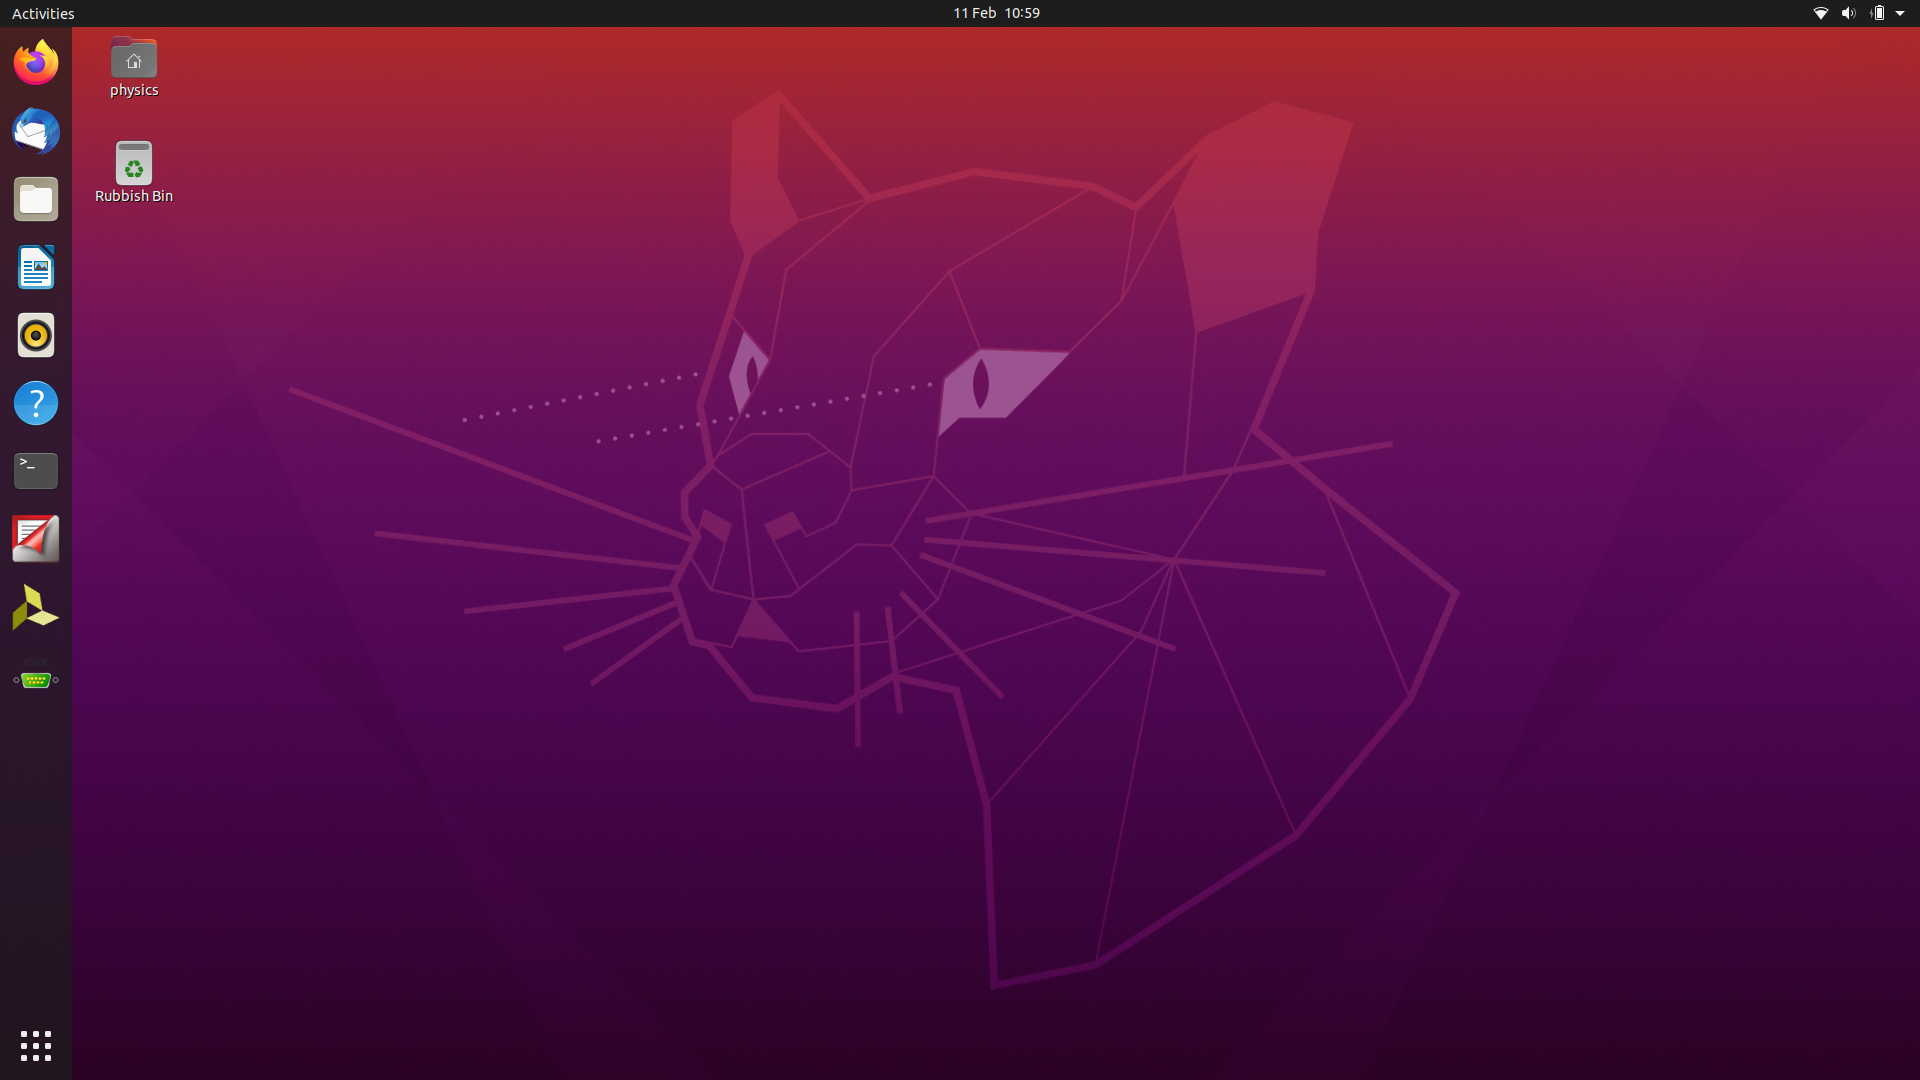
\includegraphics[width=\textwidth]{figures/blank_ubuntu_screen.png}
    \caption{A blank screen upon logging in as physics to Ubuntu}
    \label{fig:emptyscreen}
\end{figure}

You can single-left-click on any of these items to run the corresponding applications. If you run something and want to stop, just as in Windows, use the red 'x' in the top right hand corner of the window. Most windows can be resized by dragging on the corners, minimised by clicking on the underscore also in the top right corner, and expanded to full-screen mode by clicking on the rectangle in the same place. If you minimise a window belonging to one of the sidebar applications, it can be recovered by clicking again on the icon. You can also re-open a minimised icon by clicking on 'Activities' in the top left hand corner. The full set of installed applications can be seen by clicking on `nine dots' icon in the lower left corner. You can drag across the mouse pad to go up and down the full set of icons. Clicking on it again takes you back. If you are alone and want some background music or talk, the 'RythmnBox' application plays podcasts. 

The two icons in the top left of the main window are short-cuts to the Files application running on your home directory and the contents of the rubbish bin

Firefox should need no explanation. The `Files' application is like the Windows file manager, and it allows you to navigate through the hierachy of folders on the Ubuntu machine. If you right click on a file you are given an option to move to the recycle bin, just as in Windows. In fact, Ubuntu is trying to emulate the Windows operating system. The big difference between Linux and Windows is the use of the Terminal application. Windows has the DOS prompt, but DOS is so arcane that few but the brave use it very much. In Linux the Terminal 'shell' is the BASH shell, which has quite a lot of functionality and is quite sophisticated. However, you shouldn't actually need to learn too much UNIX/Linux to do this course. If you are interested, there are lots of tutorials on line in learning the BASH shell in UNIX/Linux. The serial port terminal will be useful later in the course when we are communicating with microprocessor cores on the BASYS3 board. Vivado and Vitis are the two graphical user interfaces that we will use to develop our applications. We will spend most of our time using Vivado and Vitis.

Before you can use Firefox you will need to connect your laptop to a wireless network. The icon to do this is in the top right hand corner of the screen and looks like a segment of fruit. If you click on this icon it will show you a list of available wireless networks - you should check and see that there is one that you can log in to. After logging in, the segment will be partially filled in, indicating the quality of your connection.

You should be able to use Firefox to log on to MUSE and from there with the google mail tool and Blackboard you should be able to use your laptop to take part in the lab projects without need for your own personal devices. The camera built in to the laptop and the built in microphone both work with blackboard and we will need to communicate with each other freely to make a success of the course, within the limits imposed by bandwidth.

To shut the laptop down, the small downwards arrow in the very top right pulls down a menu from which you can select the Power Off/Log Out option, and there you can do all the usual things - turn off, restart, log out, etc. In these things Ubuntu again behaves much like other popular operating systems.

There are also several other equipment items. These are, all told
\begin{enumerate}
    \item Cardboard box and packing material (please preserve in good condition)
    \item Laptop with power supply (two connected cables)
    \item Gel filled protective laptop case
    \item USB to micro-usb adaptor cable
    \item Basys3 FPGA development board
    \item PMODDAC2 two channel digital-to-analog converter (DAC) - this is small!
    \item some cables
    \item a crystal earpiece
\end{enumerate}

Obviously try not to lose anything and tell me if you do, or if anything gets broken. Try NEVER to keep drinks anywhere they can spill on the laptop. Especially on the table directly next to them. Think of them as lab equipment. You wouldn't drink in a lab, so don't keep drinks in the vicinity of this machinery.

One final thing about the laptops. If you want to dump the whole screen to a picture file, then at any time you can just press the PrtScr button which is on your keyboard two keys to the right of the space bar, and a `.png' format bitmap of the entire screen is written to the Pictures subfolder of your home directory. Try this, and then use the Files application to go to this directory, double clicking on the icon to view it. If you just want to print one window, make sure this window is selected, then hold down the Alt key and again press PrtScr (Alt-PrtScr), and a `.png' file just of the highlighted window is put in the same place. This could be useful if something isn't working right and you want to send myself or Mitch graphics that are useful in explaining your problem.

\end{document}